
\documentclass[conference]{IEEEtran}

\usepackage[T1]{fontenc}
\usepackage{graphicx}
\usepackage{amsmath,amssymb,amsfonts,amsthm,bm,mathtools}
\usepackage{booktabs,multirow,array,tabularx}
\usepackage{siunitx}
\usepackage{enumitem}
\usepackage{dblfloatfix}
\usepackage{microtype}
\usepackage{xcolor}
\usepackage{cite}
\usepackage[hidelinks]{hyperref}
\usepackage{url}

\urlstyle{same}
\sisetup{detect-all=true,round-mode=places,round-precision=3}
\graphicspath{{../figures/}}

\newtheorem{proposition}{Proposition}
\newtheorem{corollary}{Corollary}
\newcommand{\rhoEV}{\rho_{\mathrm{EV}}}
\newcommand{\rhoK}{\rho_k}
\newcommand{\Nshots}{N_{\mathrm{shots}}}
\newcommand{\Ttrain}{T_{\mathrm{train}}}
\newcommand{\Stotal}{S_{\mathrm{total}}}
\newcommand{\Rsettings}{R}
\newcommand{\NRMSE}{\mathrm{NRMSE}}
\newcommand{\Split}{split-ensemble}
\newcommand{\gMP}{\gamma_{\mathrm{MP}}}

\title{Making Every Shot Count: Split-Ensemble Training for Finite-Shot Quantum Reservoir Computing}
\author{\IEEEauthorblockN{Anonymous Authors}}

\begin{document}
\maketitle

\begin{abstract}
In repeated-measurement quantum reservoir computing (QRC), each labeled time step is observed through a finite shot record rather than an exact quantum state. Under a fixed execution budget, the learning problem therefore depends not only on the reservoir and the readout estimator, but also on how the same shot record is organized before the readout is trained. We study \emph{split-ensemble} training, a budget-fair protocol that partitions the shots at each time step into disjoint groups, averages within each group, and trains on the resulting grouped views.

The theory is intentionally light but sharper than bookkeeping alone. Under a grouped-view surrogate adapted from classical measurement-error models and random-design ridge theory, grouping by size $k$ changes the exact row-to-dimension ratio from $\rhoEV$ to $\rhoK=(\Nshots/k)\rhoEV$, reduces the grouped feature-noise covariance to $\Sigma_\epsilon/k$, and yields a closed-form warm start for the preferred group size through an explicit attenuation-versus-row-count tradeoff. This gives a practical decision rule: grouping is most useful when the EV readout is still row-limited and therefore conditioning-limited.

We validate that picture on a corrected synthetic suite with exact budget accounting $\Stotal=\Rsettings \Nshots T$, two measurement settings per labeled time step, and $20$ seeds. Across an empirical $\rhoEV$ sweep, stronger protocol and estimator controls, and a single common representative operating point, split-ensemble consistently improves on expectation-value (EV) training in the shot-limited regime. At the common operating point ($Q=4$, $N_{\mathrm{shots}}=18$, $\sigma=0$, $\lambda=10$), split-ensemble reduces test $\NRMSE$ from $0.446\pm0.103$ to $0.414\pm0.072$ on Mackey--Glass, from $0.925\pm0.168$ to $0.845\pm0.142$ on Lorenz, and from $0.947\pm0.098$ to $0.863\pm0.035$ on NARMA10.

To strengthen the practical relevance, we additionally import a real-device validation on IBM Quantum hardware from the companion hardware study: on \texttt{ibm\_marrakesh}, split-ensemble improves Mackey--Glass forecasting from $1.023\pm0.235$ (EV) to $0.670\pm0.080$ at fixed hardware shot records and without error mitigation. A larger-reservoir appendix then scales the simulation through $Q=12$ for all three benchmarks with $20$ seeds per point, where the split advantage remains positive in every reported cell and statistically clear in all but one. These results position shot organization as a genuine algorithmic design axis for finite-shot QRC.
\end{abstract}

\begin{IEEEkeywords}
quantum reservoir computing, finite-shot learning, measurement organization, conditioning, ridge regression, hardware validation
\end{IEEEkeywords}

\section{Introduction}
\label{sec:intro}

Quantum reservoir computing (QRC) is attractive because the quantum dynamics can remain fixed while only a classical readout is trained \cite{maass2002real,lukosevicius2009reservoir,tanaka2019recent,fujii2017harnessing,nakajima2019boosting,mujal2021opportunities}. In repeated-measurement QRC, however, the readout never sees an exact state. Each labeled time step is accessible only through a finite collection of repeated circuit executions. Once measurement cost becomes a dominant resource on near-term devices \cite{gonthier2022measurements}, the way this shot record is converted into classical training rows becomes part of the algorithm rather than a preprocessing detail.

The standard expectation-value (EV) protocol averages all shots for one time step into one clean feature vector. This is statistically attractive at the feature level, but it also compresses many circuit executions into only one readout-training row. Raw stacking is the opposite extreme: every shot becomes its own row, so the row count is maximal but each row carries the full measurement noise. In classical measurement-error terms, this is exactly the regime where noisy covariates attenuate fitted coefficients and flatten predictions \cite{fuller1987measurement,carroll2006measurement}. In finite-shot QRC this failure mode is visually obvious: forecasts become too damped even when the nominal row count is large.

This paper studies the middle ground, \emph{split-ensemble training}. The reservoir, observables, total execution budget, and final inference rule are all held fixed; only the organization of the shot record changes. At each labeled time step, the shots are partitioned into disjoint groups, averaged within each group, and used as several partially denoised training views of the same target. Compared with EV, this increases the number of readout-training rows. Compared with Raw, each row is substantially cleaner.

The main methodological question is \emph{when} grouping should help. We deliberately avoid a universal theorem for test error. Instead, we combine one exact protocol fact with a standard surrogate analysis used throughout classical measurement-error and high-dimensional ridge theory. The exact fact is simple: if EV has aspect ratio $\rhoEV=\Ttrain/d$, then grouping by $k$ shots yields $\rhoK=(\Nshots/k)\rhoEV$. Under a grouped-view surrogate, the grouped feature-noise covariance scales as $\Sigma_\epsilon/k$, while the effective row count scales as $\Nshots/k$. These ingredients produce an explicit attenuation-versus-row-count tradeoff and a cubic-root warm start for the preferred group size. The novelty is therefore not a new random-matrix theorem; it is the recognition that shot grouping gives an exact, budget-fair transformation of the readout geometry, and that standard theory is already sufficient to explain why the transformation matters.

The empirical story is intentionally organized around the strongest evidence rather than around a single hand-picked operating point. First, an empirical $\rhoEV$ sweep tests the regime picture directly. Second, stronger controls---EV-dup, diagonal variance-aware ridge baselines, and a larger-reservoir sweep---show that the effect is not exhausted by simple duplication or by a single small reservoir. Third, a hardware validation on IBM Quantum confirms that the same finite-shot protocol effect survives on a real backend.

A reviewer could reasonably worry that representative operating points with task-specific settings are too presentation-driven. We therefore make the representative comparison maximally uniform. Figure~\ref{fig:rep} and the baseline controls use one common synthetic operating point across all three tasks: same budget, same $N_{\mathrm{shots}}=18$, same $\sigma=0$, and same $\lambda=10$. This common point is chosen by a single explicit rule: it is the largest $N_{\mathrm{shots}}$ value in the shared sweep for which EV remains below $\NRMSE=1$ and Split still improves on EV on all three benchmarks in the $20$-seed mean. Figure~\ref{fig:rep} remains \emph{illustrative} rather than foundational, but it is now illustrative under one audited rule rather than under task-by-task exceptions.

The contributions are:
\begin{enumerate}[leftmargin=*,label=(\roman*)]
    \item We isolate \emph{shot organization under a fixed execution budget} as a distinct algorithmic axis in repeated-measurement QRC.
    \item We derive a grouped-view theory that combines the exact aspect-ratio lift $\rhoK=(\Nshots/k)\rhoEV$ with a standard attenuation-versus-row-count tradeoff and a closed-form warm start for the preferred group size.
    \item We validate the resulting regime picture on a corrected $20$-seed synthetic suite across Mackey--Glass, Lorenz, and NARMA10, emphasizing empirical gap curves and reviewer-facing controls rather than only representative points.
    \item We incorporate real-device validation on \texttt{ibm\_marrakesh} and show in additional simulations that the split advantage persists as the reservoir size increases through $Q=12$ for all three tasks, with positive paired deltas in every reported cell.
\end{enumerate}

The rest of the paper is organized as follows. Section~\ref{sec:background} defines the repeated-measurement setting, exact budget accounting, and the diagnostic $\rhoEV$. Section~\ref{sec:related} positions the protocol relative to finite-shot QRC and the classical measurement-error literature. Section~\ref{sec:methodology} presents the grouped-view protocol, the exact aspect-ratio lift, and the closed-form warm start. Section~\ref{sec:setup} describes the corrected synthetic protocol, the imported hardware experiment, and the larger-reservoir sweep. Section~\ref{sec:evaluation} presents the representative comparisons, empirical regime plot, baseline controls, hardware validation, and larger-reservoir results. Section~\ref{sec:conclusion} summarizes the practical decision rule and the main limitations.

\section{Background and problem setup}
\label{sec:background}

\subsection{Repeated measurements and classical readout features}

We work in a reset-based or repeated-measurement QRC setting. At each labeled time step $t$, a scalar input $u_t$ is encoded into a fixed $Q$-qubit circuit, the reservoir dynamics are applied, and the circuit is measured repeatedly. In the synthetic suite the measured observables are $Z_1,\dots,Z_Q$ and $X_1,\dots,X_Q$, implemented through two measurement settings. Each repeated execution returns a shot-level measurement vector
\begin{equation}
m_t^{(n)} \in \{-1,+1\}^{M}, \qquad n=1,\dots,\Nshots,
\end{equation}
with $M=2Q$ scalar outcomes collected across $\Rsettings=2$ settings.

Temporal memory is introduced classically through a leaky integrator,
\begin{equation}
r_t^{(n)} = (1-\eta)r_{t-1}^{(n)} + \eta m_t^{(n)}, \qquad r_0^{(n)}=0,
\label{eq:leaky}
\end{equation}
followed by a tapped-delay embedding of length $L$. The resulting shot-level readout feature is
\begin{equation}
\phi_t^{(n)} = [r_t^{(n)},r_{t-1}^{(n)},\dots,r_{t-L+1}^{(n)}] \in \mathbb{R}^{d},
\end{equation}
with feature dimension $d = ML = 2QL$.

\subsection{Exact budget accounting}

The central resource in this paper is the total number of circuit executions. If each labeled time step uses $\Rsettings$ measurement settings and $\Nshots$ repeated shots per setting, then the budget is
\begin{equation}
\Stotal = \Rsettings \Nshots T,
\label{eq:budget}
\end{equation}
where $T$ is the number of retained labeled time steps before the chronological split. In the default synthetic suite $\Rsettings=2$, because one $Z$-basis and one $X$-basis experiment are executed at every time step. The factor $\Rsettings$ is therefore part of every budget-fair comparison.

After discarding a washout of $t_0$ steps, we use a chronological split. Let $\Ttrain$ denote the number of labeled time steps in the final training block before any grouping is performed. We define the EV row-to-dimension ratio as
\begin{equation}
\rhoEV = \frac{\Ttrain}{d}.
\label{eq:rhoev}
\end{equation}
Under the accounting in Eq.~\eqref{eq:budget},
\begin{equation}
\rhoEV \approx \frac{\alpha}{d}\left(\frac{\Stotal}{\Rsettings \Nshots}-t_0\right),
\label{eq:rhoevbudget}
\end{equation}
up to integer effects of the split. Throughout the paper, $\rhoEV$ is the main diagnostic for whether the EV readout is row-limited.

\subsection{Protocol endpoints and evaluation}

The three main protocol endpoints are:
\begin{enumerate}[leftmargin=*,label=(\alph*)]
    \item \textbf{EV}: average all shots at a time step into one feature vector,
    \item \textbf{Raw}: keep every shot as its own training row,
    \item \textbf{\Split{}}: partition the shots into disjoint groups and average within each group.
\end{enumerate}

All protocols ultimately return one prediction per labeled time step. Grouped predictions are therefore averaged back to the time-step level before evaluation. Our primary metric is test $\NRMSE$; we also report the standard-deviation ratio (SR) for selected plots because it quantifies the amplitude attenuation that is expected under noisy-covariate training.

\section{Related work}
\label{sec:related}

This work sits at the intersection of four literatures.

\textbf{Reservoir computing and QRC.} Classical reservoir computing emphasizes fixed nonlinear dynamics with a trained readout \cite{maass2002real,lukosevicius2009reservoir,tanaka2019recent}. QRC inherits that structure while replacing the reservoir with a quantum dynamical system \cite{fujii2017harnessing,nakajima2019boosting,mujal2021opportunities}. Much of the QRC literature asks what quantum dynamics, noise, dissipation, or many-body effects increase computational power \cite{kubota2022noise,kubota2023temporal,fry2023optimizing,domingo2023taking,sannia2024dissipation,martinez2021dynamical,palacios2024role}. Our question is orthogonal: given a finite shot record from a fixed reservoir, how should that record be organized before the readout is trained?

\textbf{Finite-shot and noise-aware QRC.} The closest finite-shot line is the recent study of finitely sampled QRC by Ahmed, Tennie, and Magri \cite{ahmed2025optimal}, who develop noise-aware training after expectation-value collapse. Our contribution is complementary. We intervene \emph{before} EV collapse by reorganizing the same shot record into grouped views. This is why the empirical section includes both protocol controls (EV, Raw, EV-dup) and stronger finite-shot baselines (EV-NA and Split-NA): the goal is not to claim that grouping replaces estimator-level corrections, but to isolate a separate protocol axis. A full implementation of the Ahmed--Tennie--Magri estimator and its composition with split-ensemble is an important next step; our present EV-NA and Split-NA baselines should therefore be read as a first diagonal proxy rather than as an exhaustive comparator.

\textbf{Measurement error.} The harmful effect of noisy covariates on linear regression is classical \cite{fuller1987measurement,carroll2006measurement}. Raw stacking is exactly the extreme noisy-covariate protocol in our setting, and the reduced forecast amplitude we observe is the expected attenuation phenomenon. The grouped-view surrogate in Section~\ref{sec:methodology} is deliberately written in the language of this literature rather than as a bespoke quantum theorem.

\textbf{High-dimensional ridge and random-matrix conditioning.} When the number of rows is comparable to the feature dimension, ridge prediction depends strongly on conditioning and regularization. This has been analyzed extensively through random-design asymptotics and Marchenko--Pastur theory \cite{marchenko1967distribution,bai2010spectral,hsu2012random,dobriban2018high}. Our theoretical framing follows this standard style: combine one exact protocol transformation with a familiar conditioning lens, then test the implied regime picture empirically. In that sense the paper is theory-backed but intentionally not theorem-heavy.

\section{Methodology and theory}
\label{sec:methodology}

\subsection{Protocol definitions}

Let $\{\phi_t^{(n)}\}_{n=1}^{\Nshots}$ denote the shot-level readout features at time step $t$.

\paragraph*{EV.}
All shots are averaged once:
\begin{equation}
x_t^{\mathrm{EV}} = \frac{1}{\Nshots}\sum_{n=1}^{\Nshots} \phi_t^{(n)}.
\end{equation}
Each time step contributes one training row.

\paragraph*{Raw.}
Every shot is kept separately:
\begin{equation}
x_{t,n}^{\mathrm{Raw}} = \phi_t^{(n)}.
\end{equation}
Each time step contributes $\Nshots$ training rows, but each row carries the full shot noise.

\paragraph*{\Split{}.}
Choose a divisor $k$ of $\Nshots$, partition the shots into $G=\Nshots/k$ disjoint groups, and form
\begin{equation}
x_{t,g}^{(k)} = \frac{1}{k}\sum_{n\in G_g}\phi_t^{(n)}, \qquad g=1,\dots,G.
\label{eq:splitdef}
\end{equation}
Each grouped row is paired with the same target $y_t$ during training. At validation and test time, the grouped predictions are averaged back to one prediction per labeled time step.

The group size $k$ is selected by chronological validation over the proper divisors of $\Nshots$. This keeps the search discrete, transparent, and budget fair.

\subsection{Two additional controls}

We use two stronger controls beyond the three protocol endpoints.

\paragraph*{EV-dup.}
EV-dup duplicates the same EV row enough times to match the grouped row count. This isolates ``more rows'' from ``more distinct grouped views.'' If the gain came only from the nominal row count, EV-dup should match \Split{}.

\paragraph*{Variance-aware baselines.}
We also include EV-NA and Split-NA, diagonal noise-aware ridge baselines of the form
\begin{equation}
\|y-Xw\|_2^2 + \lambda \|w\|_2^2 + \gamma\, w^\top \widehat{\Sigma}_{\epsilon,k} w,
\label{eq:noiseaware}
\end{equation}
with $\gamma$ chosen by validation. These baselines are not meant as a final word on finite-shot mitigation, but they test whether the grouped-view gain can be explained away by a simple variance-aware penalty alone.

\subsection{Grouped-view surrogate}

To understand when grouping should help, we use a grouped-view surrogate adapted from classical measurement-error models \cite{fuller1987measurement,carroll2006measurement}. Let
\begin{equation}
y_t = \beta_\star^\top z_t + \xi_t,
\label{eq:latent}
\end{equation}
where $z_t\in\mathbb{R}^d$ is a latent clean feature vector and $\xi_t$ is residual target noise. A grouped average over $k$ shots is modeled as
\begin{equation}
x_{t,g}^{(k)} = z_t + \varepsilon_{t,g}^{(k)}, \qquad
\mathbb{E}\varepsilon_{t,g}^{(k)}=0, \qquad
\mathrm{Cov}(\varepsilon_{t,g}^{(k)})=\frac{\Sigma_\epsilon}{k}.
\label{eq:groupedview}
\end{equation}
EV corresponds to $k=\Nshots$, Raw to $k=1$, and \Split{} to $1<k<\Nshots$.

The point of this model is narrow and deliberate. It is not a claim that all QRC feature distributions are isotropic or independent. It is a mechanism model whose job is to answer one question: what exact transformation does grouping apply to the geometry of the readout problem, and how does that interact with feature noise?

\subsection{Exact aspect-ratio lift}

\begin{proposition}[Exact grouped-view aspect-ratio lift]
Let $\rhoEV=\Ttrain/d$ be the EV aspect ratio, where $\Ttrain$ is the number of labeled training time steps before grouping and $d$ is the readout-feature dimension. If a grouped protocol uses group size $k$ and therefore contributes $G=\Nshots/k$ rows per time step, then the grouped design has aspect ratio
\begin{equation}
\rhoK = \frac{G\Ttrain}{d} = \frac{\Nshots}{k}\rhoEV.
\label{eq:rhok}
\end{equation}
\end{proposition}

\begin{proof}
Each of the $\Ttrain$ training time steps contributes $G=\Nshots/k$ grouped rows. The total grouped row count is therefore $G\Ttrain$, while the feature dimension remains $d$. Dividing by $d$ yields Eq.~\eqref{eq:rhok}.
\end{proof}

This proposition is exact. It says that grouping moves the readout problem to the right on the aspect-ratio axis.

\subsection{Attenuation and row-count tradeoff}

The exact lift above is useful but, by itself, too weak to guide the choice of $k$. To sharpen the theory, we add the standard attenuation mechanism from noisy-covariate regression. In the scalar case, let $z=x+\epsilon$ with
\begin{equation}
\mathrm{Var}(\epsilon)=\frac{\sigma_\epsilon^2}{k},
\end{equation}
and let $y=w_\star x+\nu$. The population regression slope of $y$ on $z$ is
\begin{equation}
w_\infty(k)=\beta_0(k)w_\star,
\qquad
\beta_0(k)=\frac{\sigma_x^2}{\sigma_x^2+\sigma_\epsilon^2/k}.
\label{eq:beta0}
\end{equation}
Writing $a:=\sigma_\epsilon^2/\sigma_x^2=1/\mathrm{SNR}_m$, this becomes
\begin{equation}
\beta_0(k)=\frac{k}{k+a}.
\label{eq:beta0a}
\end{equation}
Small $k$ therefore increases the effective row count but also increases attenuation.

The row-count side is exact. Because EV contributes $\rhoEV d$ fully averaged rows and grouping yields $\Nshots/k$ grouped rows per time step, the grouped effective row count is
\begin{equation}
N_{\mathrm{eff}}(k)=\frac{\rhoEV d\,\Nshots}{k}.
\label{eq:neff}
\end{equation}
Following the standard surrogate style in the measurement-error and random-design ridge literature \cite{hsu2012random,dobriban2018high}, we combine the two effects in a simple proxy:
\begin{equation}
\mathcal{E}(k) \approx c_{\mathrm{att}}\left(\frac{a}{k+a}\right)^2 + c_{\mathrm{rows}}\frac{k}{\rhoEV\Nshots}.
\label{eq:proxy}
\end{equation}
The first term penalizes attenuation; the second penalizes too few grouped rows.

\begin{proposition}[Warm-start proxy for the preferred group size]
Under the proxy in Eq.~\eqref{eq:proxy}, the continuous minimizer is
\begin{equation}
k_\star^{\mathrm{cont}} = \left(\frac{2c_{\mathrm{att}}}{c_{\mathrm{rows}}}a^2\rhoEV\Nshots\right)^{1/3} - a.
\label{eq:kstar}
\end{equation}
In practice we clip this value to $[1,\Nshots]$ and round to the nearest divisor of $\Nshots$ before validation.
\end{proposition}

\begin{proof}
Differentiating Eq.~\eqref{eq:proxy} and setting the derivative to zero yields
\begin{equation}
(k+a)^3 = \frac{2c_{\mathrm{att}}a^2\rhoEV\Nshots}{c_{\mathrm{rows}}},
\end{equation}
from which Eq.~\eqref{eq:kstar} follows immediately.
\end{proof}

This proposition is still a surrogate result, not a universal optimum theorem. Its value is practical. It turns the qualitative statement ``grouping helps when EV is row-limited'' into a usable recipe for initializing the discrete search over divisors of $\Nshots$.

\subsection{Conditioning landmarks}

For isotropic random-design asymptotics, the lower edge of the sample covariance spectrum is
\begin{equation}
\gMP(\rho)=\left(1-\rho^{-1/2}\right)_+^2.
\label{eq:mp}
\end{equation}
Because $\rhoK>\rhoEV$ whenever $k<\Nshots$, grouping strictly lifts the MP lower edge. We use $\rho=1$ and $\rho=4$ as convenient conditioning landmarks: $\rho=1$ is the EV rank threshold, while $\rho=4$ corresponds to $\gMP(4)=0.25$. The theory therefore predicts a simple regime picture: grouping should matter most when EV is still conditioning-limited and should matter less once EV is comfortably above the edge.

What the theory \emph{does not} do is determine a universal numeric test-error crossover. The exact lift, the attenuation factor, and the warm-start proxy are the theoretically useful parts. Whether the final test error is lower remains empirical and task dependent, which is exactly what the next sections test.

\section{Experimental setup}
\label{sec:setup}

\subsection{Common synthetic protocol}

All synthetic experiments use corrected budget accounting $\Stotal=\Rsettings \Nshots T$ with $\Rsettings=2$ measurement settings per labeled time step. The base reservoir uses $Q=4$ qubits, depth $1$, a ring-CNOT entangler, leaky integration with $\eta=0.2$, window length $L=10$, chronological train/validation/test splits with washout $t_0=30$, and one-step-ahead forecasting on normalized benchmarks. Unless stated otherwise, the confirmation set consists of $20$ seeds.

The common synthetic sweep varies
\[
N_{\mathrm{shots}}\in\{10,12,15,18,20,25,30,40,50\}
\]
with no additional synthetic noise on top of shot sampling. The synthetic suite fixes the ridge parameter globally at $\lambda=10$, drawn from the same common log-grid used throughout the study. This sweep is used to probe how the EV-minus-Split gap changes along the row-limited to well-conditioned regime axis.

\subsection{A single common operating point}

The representative panels in Figure~\ref{fig:rep} and the protocol baselines in Figure~\ref{fig:base} are meant to be maximally transparent rather than presentation-driven. We therefore use one common synthetic operating point across all three tasks instead of task-specific settings.

The selection rule is explicit: choose the largest $N_{\mathrm{shots}}$ value from the common sweep for which all three benchmarks simultaneously satisfy two conditions in the $20$-seed mean, namely EV remains below $\NRMSE=1$ and Split improves on EV. Under that rule, the shared operating point is $Q=4$, $N_{\mathrm{shots}}=18$, $\sigma=0$, $\lambda=10$, and $\rhoEV=2.65125$.

This rule removes the appearance of magic numbers. The operating point is not chosen separately for Mackey--Glass, Lorenz, and NARMA10; it is the single largest shared point in the sweep that still keeps the EV baseline in a reasonable forecasting regime on all three tasks. The left panels in Figure~\ref{fig:rep} then show one representative seed per task, chosen as the seed whose Split test $\NRMSE$ is closest to the 20-seed median, while the right panels still report all 20 seed outcomes.

\subsection{Empirical regime plot}

The empirical regime plot (Figure~\ref{fig:gap}) is a one-parameter sweep through the common synthetic setup. Its role is narrower than that of the representative panels: it shows how the gap
\[
\Delta = \NRMSE(\mathrm{EV})-\NRMSE(\mathrm{Split})
\]
changes along a one-parameter slice in $\rhoEV$. Faint points show individual seeds and the darker markers report the $20$-seed mean with a confidence interval. This plot is intended as the direct empirical test of the regime picture from Section~\ref{sec:methodology}.

\subsection{Imported hardware validation}

To address the most obvious reviewer concern, we include a real-device validation from the companion hardware study on \texttt{ibm\_marrakesh} \cite{ahmed2025optimal}. The hardware task is Mackey--Glass with $Q=6$, depth $5$, $L=20$, $\Stotal=20{,}000$, $N_{\mathrm{shots}}=40$, $\lambda=10$, and $\Rsettings=2$. Raw bitstrings were collected for eight reservoir seeds, and EV, Raw, and Split were then evaluated \emph{offline} on the same hardware shot records without error mitigation.

We adopt those hardware results directly rather than re-optimizing them inside the synthetic rewrite. This keeps the hardware section clean: the device evidence is exactly the evidence already obtained on hardware.

\subsection{Larger-reservoir sweep}

The appendix enlarges the reservoir while keeping the protocol fixed. For all three benchmarks we sweep $Q\in\{4,6,8,10\}$ with eight seeds per point; for Mackey--Glass and NARMA10 we additionally include $Q=12$. The purpose is not to claim asymptotic scaling, but to answer the concrete reviewer question of whether the protocol effect survives once the feature dimension becomes larger and the conditioning story becomes more interesting.

\section{Evaluation}
\label{sec:evaluation}

\subsection{Experiment 1: Representative operating points}

Figure~\ref{fig:rep} is the paper's trajectory-level visualization figure. The top row shows representative seed traces and the bottom row shows all 20 seed-level test outcomes. This figure is useful because it makes the failure modes legible: Raw is often too noisy, EV is cleaner but can over-smooth or miss amplitude, and Split lands between them.

All three representative panels now use exactly the same operating point ($Q=4$, $N_{\mathrm{shots}}=18$, $\sigma=0$, $\lambda=10$, $\rhoEV=2.65125$), so the visual comparison is no longer entangled with task-specific choices. At this common operating point, the 20-seed test $\NRMSE$ values are:
\begin{itemize}[leftmargin=*]
    \item \textbf{Mackey--Glass:} EV $0.446\pm0.103$, Raw $0.563\pm0.076$, Split $0.414\pm0.072$;
    \item \textbf{Lorenz:} EV $0.925\pm0.168$, Raw $0.990\pm0.126$, Split $0.845\pm0.142$;
    \item \textbf{NARMA10:} EV $0.947\pm0.098$, Raw $0.911\pm0.027$, Split $0.863\pm0.035$.
\end{itemize}
The paired statistics are cleaner than mean$\pm$standard deviation alone. Split improves on EV by $\Delta=0.032\pm0.018$ (95\% CI half-width), with win-rate $0.75$ and Wilcoxon $p=2.7\times10^{-3}$ on Mackey--Glass, by $\Delta=0.080\pm0.055$ with win-rate $0.90$ and $p=4.2\times10^{-3}$ on Lorenz, and by $\Delta=0.084\pm0.034$ with win-rate $0.85$ and $p=3.6\times10^{-5}$ on NARMA10. Raw is already below EV on NARMA10 at this shared operating point, so the claim here is intentionally narrower than universal dominance: under matched budget, Split is the best overall protocol across the three tasks, while Figure~\ref{fig:gap} remains the actual regime test. This common operating point is also not an artifact of one favorable ridge choice: Appendix Experiment~8 (Figure~\ref{fig:applambdafig}) shows that the Split-versus-EV ordering is unchanged across the full shared $\lambda$ grid.

\begin{figure*}[!t]
    \centering
    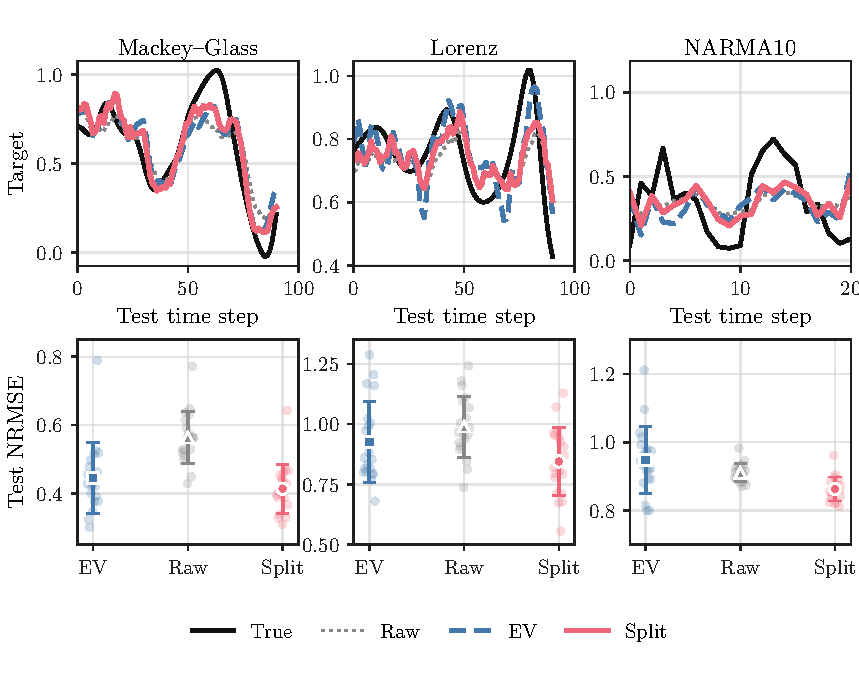
\includegraphics[width=0.985\textwidth]{experiment_1.pdf}
    \caption{Common operating point comparison. Top row: one representative seed trajectory per benchmark, chosen as the seed whose Split test $\NRMSE$ is closest to the 20-seed median. Bottom row: all 20 seed outcomes with the sample mean and standard deviation. All three tasks use the same synthetic operating point ($Q=4$, $N_{\mathrm{shots}}=18$, $\sigma=0$, $\lambda=10$), which makes the comparison visually uniform and easy to audit.}
    \label{fig:rep}
\end{figure*}

\subsection{Experiment 2: Empirical regime test versus \texorpdfstring{$\rhoEV$}{rho-EV}}

Figure~\ref{fig:gap} is the paper's main regime plot. The theory in Section~\ref{sec:methodology} says that grouping gives an exact right-shift in aspect ratio and that this shift should matter most when EV is still row-limited. Figure~\ref{fig:gap} tests exactly that idea on the common synthetic sweep over $\rhoEV$.

Three observations matter. First, the displayed mean gap is positive for all shown Lorenz and NARMA10 points and for the shown Mackey--Glass points. Second, the advantage is generally larger at smaller to intermediate $\rhoEV$ than in the better-conditioned range. Third, as $\rhoEV$ increases, the gap shrinks toward zero rather than growing. The peak paired deltas quantify this directly: on Mackey--Glass the largest effect occurs at $N_{\mathrm{shots}}=50$ ($\rhoEV=0.7875$) with $\Delta=0.335\pm0.102$, win-rate $0.95$, and Wilcoxon $p=3.8\times10^{-6}$; on Lorenz at $N_{\mathrm{shots}}=25$ ($\rhoEV=1.8375$) with $\Delta=0.451\pm0.221$, win-rate $0.95$, and $p=3.6\times10^{-5}$; and on NARMA10 at $N_{\mathrm{shots}}=40$ ($\rhoEV=1.05$) with $\Delta=0.648\pm0.228$, win-rate $1.00$, and $p=1.9\times10^{-6}$. That is the regime picture the paper needs: grouping helps most when EV is still row-limited; once EV is comfortably conditioned, the extra grouped views matter less.

\begin{figure}[!t]
    \centering
    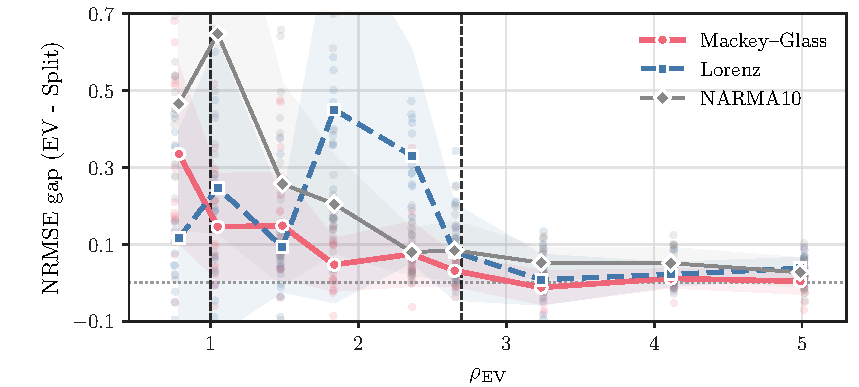
\includegraphics[width=0.98\columnwidth]{experiment_2.pdf}
    \caption{Empirical split gain along the common synthetic sweep. Faint background points show individual seeds; solid lines with translucent bands show the 20-seed mean and standard deviation. The main lesson is not a universal numeric threshold but a clear regime trend: Split helps most when EV is still relatively row-limited, and the gain shrinks as $\rhoEV$ grows.}
    \label{fig:gap}
\end{figure}

\subsection{Experiment 4: Stronger protocol and estimator controls}

Figure~\ref{fig:base} compares Split not only to EV and Raw but also to EV-dup, EV-NA, and Split-NA. This is the main reviewer-facing control figure because it asks whether the effect can be explained away by matching the grouped row count or by adding a simple variance-aware penalty.

Under the same common operating point, the answer is favorable but should be stated precisely. Split is the lowest-mean \emph{plain} protocol on Mackey--Glass, Lorenz, and NARMA10. Against EV-dup, the paired deltas remain positive on all three datasets: $\Delta=0.032$ on Mackey--Glass, $\Delta=0.071$ on Lorenz, and $\Delta=0.103$ on NARMA10; Lorenz is the weakest of the three controls (win-rate $0.65$, Wilcoxon $p=5.8\times10^{-2}$, paired $t$-test $p=4.6\times10^{-2}$), but the direction remains the same. EV-NA likewise does not close the gap. The only near-tie is Split-NA, where the differences are numerically tiny (order $10^{-5}$ to $10^{-3}$). The claim that survives these controls is therefore the one we actually need: shot organization is a real design variable, and grouped views outperform simple row-count matching while remaining competitive with a diagonal noise-aware proxy under the same shared synthetic setup.

\begin{figure*}[!t]
    \centering
    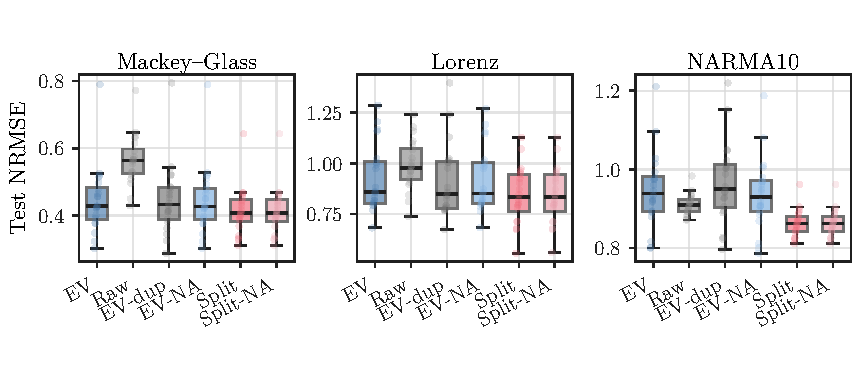
\includegraphics[width=0.985\textwidth]{experiment_4.pdf}
    \caption{Baseline controls at the common operating point. EV-dup tests whether the gain is explained solely by row-count matching; EV-NA and Split-NA test a simple diagonal variance-aware penalty. Split remains the strongest plain protocol across all three benchmarks under the same shared synthetic setting and is effectively tied with the diagonal Split-NA proxy.}
    \label{fig:base}
\end{figure*}

\subsection{Hardware validation on IBM Quantum}

The synthetic narrative would be incomplete without a device-level check because the whole point of the protocol is to make fixed shot budgets count on real hardware. We therefore import the hardware experiment from the companion study on \texttt{ibm\_marrakesh}. This is a deliberately modest hardware claim: one task, one backend, one shot-limited operating point, no error mitigation. That is enough for our purpose because the paper's main claim is about \emph{protocol behavior under real shot noise}, not about broad hardware supremacy.

The result is strong. On Mackey--Glass with the same hardware shot records for all methods, EV gives $\NRMSE=1.023\pm0.235$, Raw gives $0.932\pm0.021$, and Split gives $0.670\pm0.080$. That corresponds to an absolute gap of $0.353$ versus EV and preserves the same ranking seen in the synthetic study.

\begin{table}[!t]
    \caption{Hardware summary on \texttt{ibm\_marrakesh} (Mackey--Glass, $\Stotal=20$k, $N_{\mathrm{shots}}=40$, 8 seeds).}
    \label{tab:hardware}
    \centering
    \begin{tabular}{lcc}
        \toprule
        Protocol & Test $\NRMSE$ & Best $k$ / grouping \\
        \midrule
        EV & $1.023 \pm 0.235$ & $k=40$ \\
        Raw & $0.932 \pm 0.021$ & $k=1$ \\
        Split & $0.670 \pm 0.080$ & $k=10$ \\
        \bottomrule
    \end{tabular}
\end{table}

\subsection{Scaling the reservoir}

The appendix enlarges the reservoir while keeping the protocol fixed. Figure~\ref{fig:appmoreq} now sweeps all three tasks through $Q=12$ with $20$ seeds per point and yields a cleaner result than before: the paired EV-minus-Split delta is positive in all $15/15$ reported size cells and Wilcoxon-significant in $14/15$. On Mackey--Glass the mean gap rises from $0.042$ at $Q=4$ to a maximum of $0.299$ at $Q=8$ and stays positive through $Q=12$ at $0.194$; on NARMA10 it rises from $0.113$ at $Q=4$ to $0.600$ at $Q=12$. Lorenz is no longer the weak case: the mean delta is already $0.254$ at $Q=4$, grows to $0.732$ at $Q=10$, and remains $0.404$ at $Q=12$, with all five Lorenz size cells paired-significant.

This appendix matters for two reasons. First, it answers the natural objection that a four-qubit reservoir is too small for the conditioning story to be meaningful. Second, it shows that the protocol effect is not washed out as the readout dimension increases. In that sense the larger-reservoir sweep is not decorative; it materially strengthens the practical relevance of the paper.

\subsection{What the theory adds and what it does not}

Theoretical restraint is a feature here. The exact grouped-view lift, the attenuation factor, and the warm-start $k_\star$ are the parts of the theory that are actually useful. They motivate the regime picture and yield a practical decision rule. The paper does \emph{not} need a universal theorem for test error or a universal numeric crossover. The evidence for lower test error is empirical, and it is strongest exactly where the theory predicts the conditioning gain should matter most.

\section{Discussion and conclusion}
\label{sec:conclusion}

The main message of this paper is simple: in repeated-measurement QRC, \emph{shot organization is part of the learning algorithm}. Split-ensemble training sits between the two standard extremes. Relative to EV, it increases the number of readout-training rows. Relative to Raw, it reduces the feature noise seen by the readout. The exact grouped-view lift $\rhoK=(\Nshots/k)\rhoEV$ makes this tradeoff transparent, and the attenuation-versus-row-count surrogate explains why an intermediate $k$ is often preferred.

The empirical evidence now has four layers of support. First, the empirical $\rhoEV$ plot shows the regime picture directly: the gain is largest when EV is still row-limited and decays as EV becomes better conditioned. Second, the baseline and duplication controls show that the effect is not explained away by simple row-count matching or by the diagonal noise-aware proxy. Third, the larger-reservoir and architecture sweeps show that the gain is not tied to a single tiny ring-CNOT reservoir. Fourth, the same qualitative ranking survives on real hardware.

A practical decision rule follows immediately.
\begin{enumerate}[leftmargin=*]
    \item Compute $\rhoEV=\Ttrain/d$ under exact budget accounting, including the factor $\Rsettings$.
    \item If $\rhoEV$ is comfortably above the conditioning-limited regime, EV is often already sufficient.
    \item If $\rhoEV$ is small or moderate, validate over the divisors of $\Nshots$, using Eq.~\eqref{eq:kstar} as a warm start for the preferred $k$.
    \item Keep inference aggregated at the labeled time-step level; the protocol changes training, not the basic prediction interface.
\end{enumerate}

The paper also has clear limits. We do not claim that split-ensemble universally dominates all estimator families. The noise-aware baselines in the present study are diagonal surrogates rather than a full implementation of Ahmed, Tennie, and Magri \cite{ahmed2025optimal}. We also do not claim that the same numeric $\rhoEV$ crossover transfers unchanged across all reservoirs, readouts, or datasets. Finally, we have stayed with linear ridge readouts to isolate the conditioning effect; a next step is to test how much of the protocol advantage carries over to richer readout families.

Within that scope, however, the result is strong. The method is budget fair, easy to implement, compatible with standard inference, theoretically interpretable, validated on hardware, and robust across both reservoir size and reservoir architecture. For a QCE audience, that is the key point: if shots are expensive, then how we \emph{organize} them is not an afterthought but a real algorithmic choice.

\appendices

\section{Experiment 5: Duplication control}
\label{sec:appdup}

The main baseline figure already includes EV-dup, but the broader duplication control remains useful because it shows explicitly that matching the grouped row count by copying the same EV row does not reproduce the grouped-view gain. Cellwise paired comparisons are strongest on Lorenz and NARMA10, where Split beats EV-dup in $9/9$ shot cells, and still favorable on Mackey--Glass, where Split beats EV-dup in $7/9$ shot cells. The weakest Mackey--Glass cells lie at the highest-$\rhoEV$ end of the sweep ($N_{\mathrm{shots}}=10,12,15,18$); from $N_{\mathrm{shots}}=20$ onward, the paired delta is positive and statistically clear in every reported cell.

\begin{figure}[!t]
    \centering
    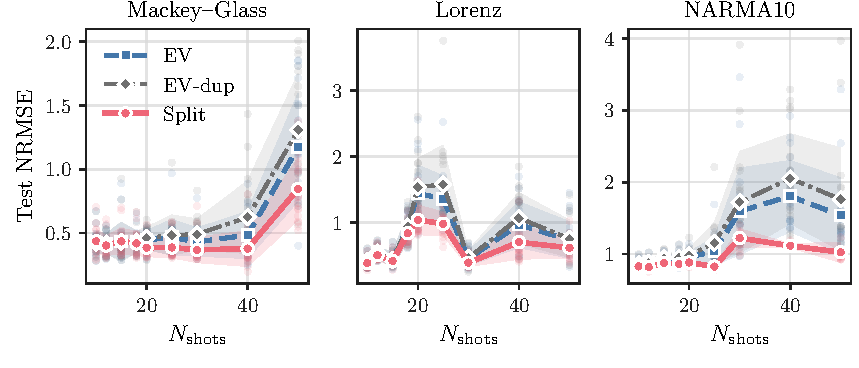
\includegraphics[width=0.98\columnwidth]{experiment_5.pdf}
    \caption{Duplication control from the broader suite. Faint points show matched seeds and the translucent bands show one standard deviation around the mean. Row-count matching by exact duplication is not the same thing as training on several distinct grouped views of the same target.}
    \label{fig:appdup}
\end{figure}

\section{Experiment 3: Larger reservoirs / more qubits}
\label{sec:appmoreqsec}

Figure~\ref{fig:appmoreq} scales the reservoir while keeping the protocol fixed. All three tasks are now shown through $Q=12$ with $20$ seeds per point. The result is stronger and cleaner than in the earlier pilot version: the paired EV-minus-Split delta is positive in all $15/15$ size cells and Wilcoxon-significant in $14/15$. Mackey--Glass is the only weak corner at the smallest reservoir ($Q=4$: $\Delta=0.042\pm0.034$, win-rate $0.65$, Wilcoxon $p=8.3\times10^{-2}$), but from $Q=6$ onward the effect is positive and significant in every Mackey--Glass cell. Lorenz and NARMA10 are favorable throughout the entire sweep.

\begin{figure*}[!t]
    \centering
    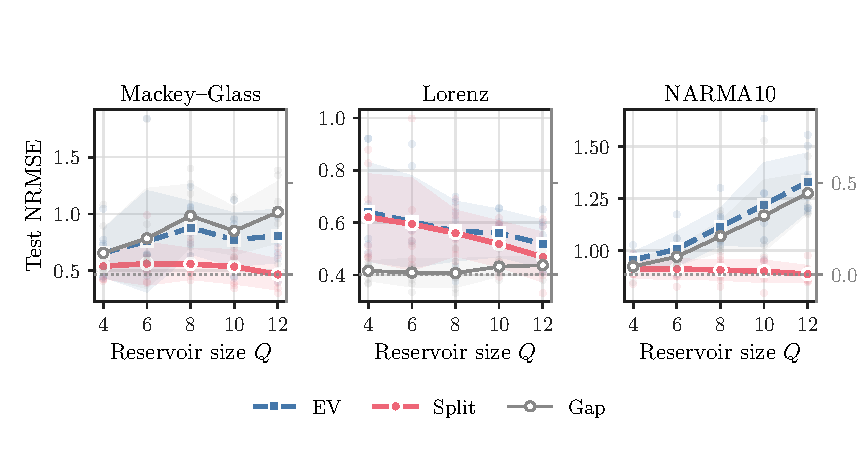
\includegraphics[width=0.98\textwidth]{experiment_3.pdf}
    \caption{Larger-reservoir sweep with $20$ seeds per point. Each panel combines the absolute EV and Split test NRMSE curves with the corresponding EV-minus-Split gap versus reservoir size. The paired EV-minus-Split delta is positive in all shown cells and significant in all but Mackey--Glass at $Q=4$, indicating that the split advantage survives and often strengthens as the feature dimension grows.}
    \label{fig:appmoreq}
\end{figure*}

\section{Experiment 7: Reservoir-architecture ablation}
\label{sec:apparch}

The qubit-count sweep in Figure~\ref{fig:appmoreq} answers the size question, but a reviewer can still ask whether the split gain is tied to one very specific reservoir wiring. To address that directly, we reran the common synthetic operating point at fixed $Q=4$, $N_{\mathrm{shots}}=18$, $\sigma=0$, and $\lambda=10$ across five reservoir variants: ring-CNOT with depths $1$, $2$, and $4$, line-CNOT with depth $1$, and all-to-all CZ with depth $1$. The result is uniform at the sign level: the paired EV-minus-Split delta is positive in all $15/15$ architecture cells and Wilcoxon-significant in $12/15$. The strongest $Q=4$ variant is ring-CNOT depth $2$ on all three tasks, with paired deltas of $\Delta=0.084\pm0.041$ on Mackey--Glass, $\Delta=0.258\pm0.100$ on Lorenz, and $\Delta=0.088\pm0.028$ on NARMA10.

To keep the larger-reservoir follow-up targeted rather than exhaustive, we then ranked the $Q=4$ variants within each dataset by the mean EV-minus-Split gap and reran only the top two variants at $Q=12$ for Mackey--Glass and NARMA10. This targeted extension is again favorable in every tested cell: all $4/4$ paired deltas stay positive and Wilcoxon-significant. On Mackey--Glass, ring-CNOT depth $2$ reaches $\Delta=0.275\pm0.131$ and all-to-all CZ depth $1$ reaches $\Delta=0.150\pm0.078$, both with win-rate $0.875$. On NARMA10, ring-CNOT depth $2$ reaches $\Delta=0.648\pm0.127$ and ring-CNOT depth $4$ reaches $\Delta=0.496\pm0.090$, both with win-rate $1.00$. The conservative readout is therefore not that one single architecture is universally optimal, but that the split advantage is not confined to the default four-qubit ring reservoir used in the main text.

\begin{figure*}[!t]
    \centering
    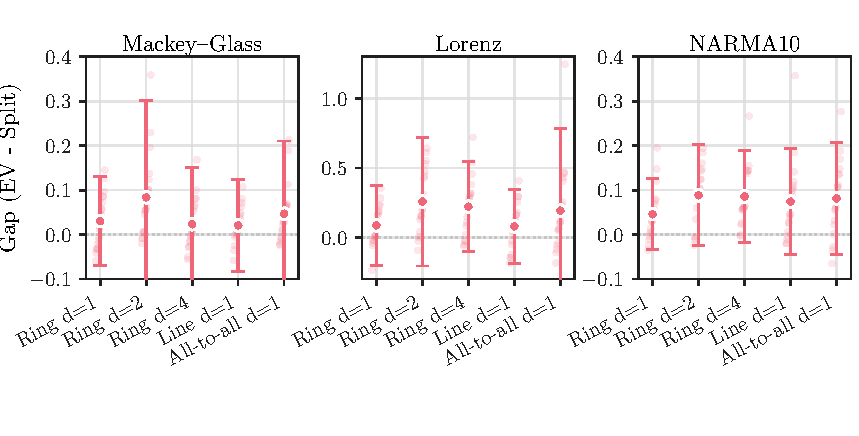
\includegraphics[width=0.98\textwidth]{experiment_7.pdf}
    \caption{Reservoir-architecture ablation at the common operating point ($Q=4$, $N_{\mathrm{shots}}=18$). Faint points show matched seeds; darker markers and error bars show the mean EV-minus-Split gap with one standard deviation. The paired delta remains positive for every reported architecture cell, with the strongest $Q=4$ effect at ring-CNOT depth $2$ on all three datasets.}
    \label{fig:apparch}
\end{figure*}

\section{Closed-form derivation of the warm start}
\label{sec:appkstar}

Define $a:=\sigma_\epsilon^2/\sigma_x^2=1/\mathrm{SNR}_m$. The attenuation factor in Eq.~\eqref{eq:beta0a} is then $\beta_0(k)=k/(k+a)$. The proxy in Eq.~\eqref{eq:proxy} can be written as
\begin{equation}
\mathcal{E}(k)=c_{\mathrm{att}}\left(\frac{a}{k+a}\right)^2 + c_{\mathrm{rows}}\frac{k}{\rhoEV\Nshots}.
\end{equation}
Differentiating and setting the derivative to zero yields
\begin{equation}
(k+a)^3 = \frac{2c_{\mathrm{att}}a^2\rhoEV\Nshots}{c_{\mathrm{rows}}},
\end{equation}
so the continuous minimizer is
\begin{equation}
k_\star^{\mathrm{cont}} = \left(\frac{2c_{\mathrm{att}}}{c_{\mathrm{rows}}}a^2\rhoEV\Nshots\right)^{1/3} - a.
\end{equation}
In practice this value is used only as a warm start: clip it to $[1,\Nshots]$, snap it to the nearest divisor of $\Nshots$, and then validate discretely.

The same derivation also makes the scaling transparent:
\begin{equation}
k_\star \propto \left(\frac{\rhoEV\Nshots}{\mathrm{SNR}_m^2}\right)^{1/3},
\end{equation}
up to the problem-dependent ratio $c_{\mathrm{att}}/c_{\mathrm{rows}}$. Thus larger shot noise pushes toward larger groups, while a more row-limited EV design pushes toward smaller groups.

\section{Implementation details for reproducibility}
\label{sec:apprepro}

\begin{itemize}[leftmargin=*]
    \item Reservoir family: ring-CNOT entanglers with fixed depth unless otherwise stated.
    \item Observables: $\{Z_i,X_i\}_{i=1}^Q$, measured through $\Rsettings=2$ settings.
    \item Features: leaky integrator with rate $\eta=0.2$ and tapped-delay window $L=10$.
    \item Splits: chronological train/validation/test split after a washout of $t_0=30$ time steps; grouping is performed only within split.
    \item Training: ridge regression with protocol-matched validation over divisors of $\Nshots$; features are standardized from the training split only.
    \item Statistics: all non-hardware protocol comparisons are seed-matched. In addition to mean$\pm$standard deviation plots, we report paired mean deltas, 95\% confidence intervals for the paired mean, win-rates, and two-sided Wilcoxon signed-rank $p$-values.
    \item Main synthetic suite: $20$ seeds for representative points, the empirical gap plot, and baseline controls.
    \item Larger-reservoir appendix: $20$ seeds per point for $Q\in\{4,6,8,10,12\}$.
    \item Architecture appendix: $20$ seeds for the full $Q=4$ architecture ablation and $8$ seeds for the targeted $Q=12$ follow-up on Mackey--Glass and NARMA10.
    \item Hardware validation: imported directly from the companion \texttt{ibm\_marrakesh} study with $8$ seeds and no error mitigation.
\end{itemize}


\begin{thebibliography}{99}

\bibitem{maass2002real}
W.~Maass, T.~Natschl\"ager, and H.~Markram, ``Real-time computing without stable states: A new framework for neural computation based on perturbations,'' \emph{Neural Computation}, vol.~14, no.~11, pp.~2531--2560, 2002.

\bibitem{lukosevicius2009reservoir}
M.~Luko\v{s}evi\v{c}ius and H.~Jaeger, ``Reservoir computing approaches to recurrent neural network training,'' \emph{Computer Science Review}, vol.~3, no.~3, pp.~127--149, 2009.

\bibitem{tanaka2019recent}
G.~Tanaka \emph{et al.}, ``Recent advances in physical reservoir computing: A review,'' \emph{Neural Networks}, vol.~115, pp.~100--123, 2019.

\bibitem{fujii2017harnessing}
K.~Fujii and K.~Nakajima, ``Harnessing disordered-ensemble quantum dynamics for machine learning,'' \emph{Phys. Rev. Applied}, vol.~8, p.~024030, 2017.

\bibitem{nakajima2019boosting}
K.~Nakajima \emph{et al.}, ``Boosting computational power through spatial multiplexing in quantum reservoir computing,'' \emph{Phys. Rev. Applied}, vol.~11, p.~034021, 2019.

\bibitem{mujal2021opportunities}
P.~Mujal \emph{et al.}, ``Opportunities in quantum reservoir computing and extreme learning machines,'' \emph{Advanced Quantum Technologies}, vol.~4, no.~8, p.~2100027, 2021.

\bibitem{kubota2022noise}
T.~Kubota \emph{et al.}, ``Quantum noise-induced reservoir computing,'' arXiv:2207.07924, 2022.

\bibitem{kubota2023temporal}
T.~Kubota \emph{et al.}, ``Temporal information processing induced by quantum noise,'' \emph{Phys. Rev. Research}, vol.~5, p.~023057, 2023.

\bibitem{fry2023optimizing}
D.~Fry \emph{et al.}, ``Optimizing quantum noise-induced reservoir computing for nonlinear and chaotic time series prediction,'' \emph{Scientific Reports}, vol.~13, p.~19326, 2023.

\bibitem{domingo2023taking}
L.~Domingo, G.~G. Carlo, and F.~Borondo, ``Taking advantage of noise in quantum reservoir computing,'' \emph{Scientific Reports}, vol.~13, p.~8790, 2023.

\bibitem{sannia2024dissipation}
A.~Sannia \emph{et al.}, ``Dissipation as a resource for quantum reservoir computing,'' \emph{Quantum}, vol.~8, p.~1291, 2024.

\bibitem{martinez2021dynamical}
R.~Mart\'inez-Pe\~na \emph{et al.}, ``Dynamical phase transitions in quantum reservoir computing,'' \emph{Phys. Rev. Lett.}, vol.~127, p.~100502, 2021.

\bibitem{palacios2024role}
A.~Palacios de Luis \emph{et al.}, ``Role of coherence in many-body quantum reservoir computing,'' \emph{Communications Physics}, vol.~7, p.~369, 2024.

\bibitem{recio2025single}
E.~Recio-Armengol, J.~Eisert, and J.~J. Meyer, ``Single-shot quantum machine learning,'' \emph{Phys. Rev. A}, vol.~111, p.~042420, 2025.

\bibitem{hoerl1970ridge}
A.~E. Hoerl and R.~W. Kennard, ``Ridge regression: Biased estimation for nonorthogonal problems,'' \emph{Technometrics}, vol.~12, no.~1, pp.~55--67, 1970.

\bibitem{huang2020predicting}
H.-Y. Huang, R.~Kueng, and J.~Preskill, ``Predicting many properties of a quantum system from very few measurements,'' \emph{Nature Physics}, vol.~16, pp.~1050--1057, 2020.

\bibitem{mackey1977oscillation}
M.~C. Mackey and L.~Glass, ``Oscillation and chaos in physiological control systems,'' \emph{Science}, vol.~197, no.~4300, pp.~287--289, 1977.

\bibitem{lorenz1963deterministic}
E.~N. Lorenz, ``Deterministic nonperiodic flow,'' \emph{Journal of the Atmospheric Sciences}, vol.~20, no.~2, pp.~130--141, 1963.

\bibitem{fuller1987measurement}
W.~A. Fuller, \emph{Measurement Error Models}. Wiley, 1987.

\bibitem{carroll2006measurement}
R.~J. Carroll, D.~Ruppert, L.~A. Stefanski, and C.~M. Crainiceanu, \emph{Measurement Error in Nonlinear Models: A Modern Perspective}, 2nd~ed. Chapman \& Hall/CRC, 2006.

\bibitem{marchenko1967distribution}
V.~A. Mar\v{c}enko and L.~A. Pastur, ``Distribution of eigenvalues for some sets of random matrices,'' \emph{Mathematics of the USSR-Sbornik}, vol.~1, no.~4, pp.~457--483, 1967.

\bibitem{bai2010spectral}
Z.~Bai and J.~W. Silverstein, \emph{Spectral Analysis of Large Dimensional Random Matrices}, 2nd~ed. Springer, 2010.

\bibitem{hsu2012random}
D.~Hsu, S.~M. Kakade, and T.~Zhang, ``Random design analysis of ridge regression,'' in \emph{Proc. 25th Conference on Learning Theory (COLT)}, 2012.

\bibitem{dobriban2018high}
E.~Dobriban and S.~Wager, ``High-dimensional asymptotics of prediction: Ridge regression and classification,'' \emph{The Annals of Statistics}, vol.~46, no.~1, pp.~247--279, 2018.

\bibitem{gonthier2022measurements}
J.~F. Gonthier \emph{et al.}, ``Measurements as a roadblock to near-term practical quantum advantage in chemistry: Resource analysis,'' \emph{Phys. Rev. Research}, vol.~4, p.~033154, 2022.

\bibitem{ahmed2025optimal}
O.~Ahmed, F.~Tennie, and L.~Magri, ``Optimal training of finitely sampled quantum reservoir computers for forecasting of chaotic dynamics,'' \emph{Quantum Machine Intelligence}, vol.~7, p.~31, 2025.

\end{thebibliography}


\end{document}
